		\documentclass[]{article}
		\usepackage{amsmath}
		\usepackage{graphicx}
		\usepackage{float}
		%opening
		\title{NCTU Machine Learning Hw2}
		\author{Liang Yu Pan 0486016}
		
		\begin{document}
			
			\maketitle
			\section{Information Theory}
			
				\subsection*{(a)}
					\paragraph{Overview}
					We use the differential entropy theorem with \textbf{Lagrange multipliers} to prove that the probability distribution which maximize the differential entropy is \textbf{Gaussian distribution}.
				\paragraph{Useful formula}
						\begin{align}
					H(x) &= -\int p(x)\ln{p(x)} dx\\
					\int_{-\infty}^{\infty} p(x) dx &= 1\\
					\int_{-\infty}^{\infty} x p(x) dx &= \mu\\
				    \int_{-\infty}^{\infty} (x - \mu)^{2} p(x) dx &= \sigma^{2}
					\end{align}
				\paragraph{Solve p(x)}
						By \textbf{Lagrange multipliers} and formula(1),(2),(3),(4), we get the formula 
						\begin{align}
						L &= - \int_{-\infty}^{\infty} p(x)\ln{p(x)} dx + \lambda_{1}(\int_{-\infty}^{\infty} p(x) dx - 1) + \lambda_{2}(\int_{-\infty}^{\infty} xp(x) dx - \mu) + \lambda_{3}(\int_{-\infty}^{\infty} (x - \mu)^{2} p(x) dx - \sigma^{2})			
		\end{align}								
		
						
						Then solve $\frac{\delta{L}}{\delta{p(x)}} = 0$, $\frac{\delta{L}}{\delta{p(x)}} = -\ln{p(x)} - 1 + \lambda_{1} + \lambda_{2} x + \lambda_{3}(x - \mu)^{2}$
						
						We get 
						\begin{align}
						p(x) &= e^{- 1 + \lambda_{1} + \lambda_{2} x + \lambda_{3}(x - \mu)^{2}}				
		\end{align}								
		
						
						Substitute (6) into (2), (3), (4), we can get 
						\begin{align}
						\lambda_{1} &= 1 - \frac{1}{2} \ln{2\pi \sigma^{2}}\\
						\lambda_{2} &= 0\\
						\lambda_{3} &= \frac{1}{2\sigma^{2}}  
						\end{align}
						
						Then substitute (7),(8),(9) into (5), we can get
						\begin{align}
						p(x) &= \frac{1}{2\pi\sigma^{2}}e^{-\frac{(x-\mu)^{2}}{2\sigma^{2}}}
						\end{align}
						which is \textbf{Gaussian distribution}.
		\subsection*{(b)}
				\paragraph*{derive entropy}
				Substitute (10) into (1), we get $\frac{1}{2}(\ln{2\pi\sigma^{2}}+1)$
						\section{Bayesian Inference for the Gaussian}
						\subsection*{(a)}
							\paragraph*{Overview}
								Because that $Posterior \propto Likelihood \times Prior$, then $\Lambda_{MAP}$ can solved by $argmax_{\Lambda}(Posterior)$.													\paragraph*{Solve Posterior}
								\begin{align}
								Prior:W(\Lambda|W_{0},V_{0}) &= B|\Lambda|^{\frac{V_{0}-D-1}{2}}e^{-\frac{1}{2}tr(W_{0}^{-1}\Lambda)}\\
								B(W_{0},V_{0}) &= |W_{0}|^{-\frac{V_{0}}{2}}[2^{\frac{V_{0}D}{2}}\pi^{\frac{D(D-1)}{4}}\prod_{i=1}^{D}\Gamma(\frac{V_{0}+1-i}{2})]^{-1}, D=2\\
								Likelihood:\prod_{n=1}^{N}N(X_{n}|\mu,\Lambda^{-1}) &\propto |\Lambda|^{\frac{N}{2}}e^{-\frac{1}{2}tr(\Lambda S)}\\
								S &= \Sigma_{n}(X_{n}-\mu)(X_{n}-\mu)^{T}
								\end{align}
								By (11), (13), we can get $Posterior \propto |\Lambda|^{\frac{V_{0}-D-1+N}{2}}e^{-\frac{1}{2}tr((W_{0}^{-1}+S)\Lambda)}$				
									\paragraph*{Solve $\Lambda_{MAP}$}
									To $argmax_{\Lambda}(Posterior)$, we solve $\frac{\partial{\Lambda_{MAP}}}{\partial{\Lambda}} = 0$
									We get $\Lambda_{MAP} = (V_{0}+N-D-1)(W_{0}^{-1}+S)^{-1}$			
									\subsection*{(b)}\mbox{}\\
										\begin{figure}[H]
											\centering
											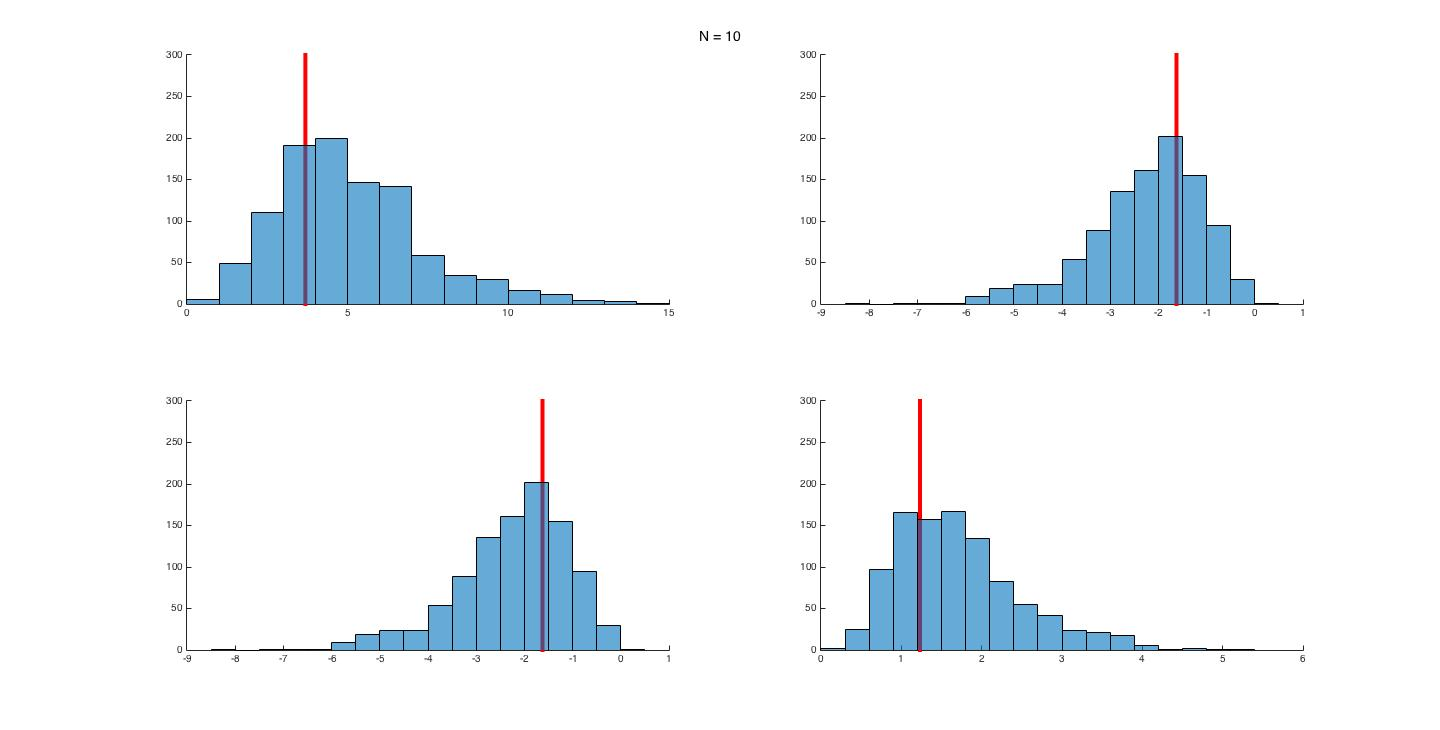
\includegraphics[width=1.2\linewidth]{2b1}
											\caption{1000 samples wishart distribution for N=10}
											\label{fig:2b1}
										\end{figure}	
										\begin{figure}[H]
											\centering
											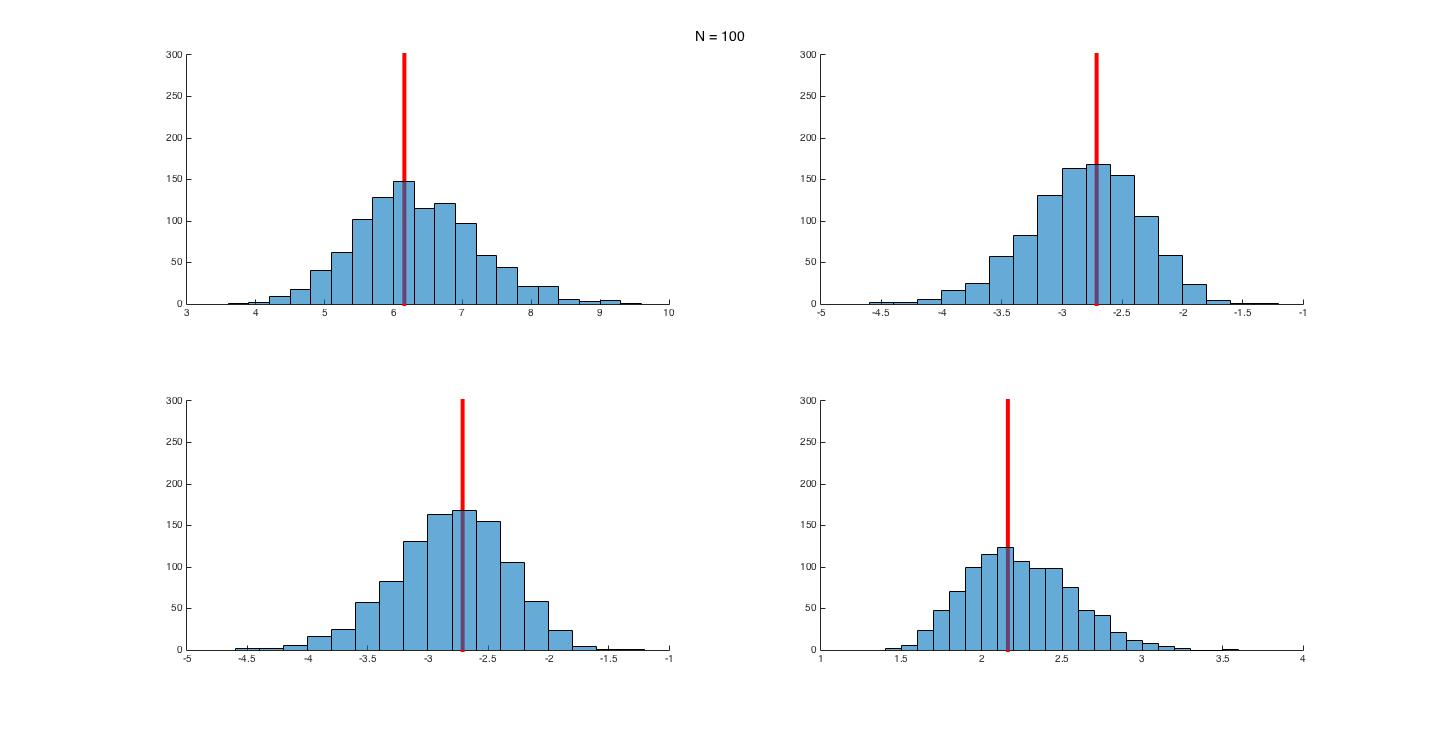
\includegraphics[width=1.2\linewidth]{2b2}
											\caption{1000 samples wishart distribution for N=100}
											\label{fig:2b2}
										\end{figure}	
										\begin{figure}[H]
											\centering
											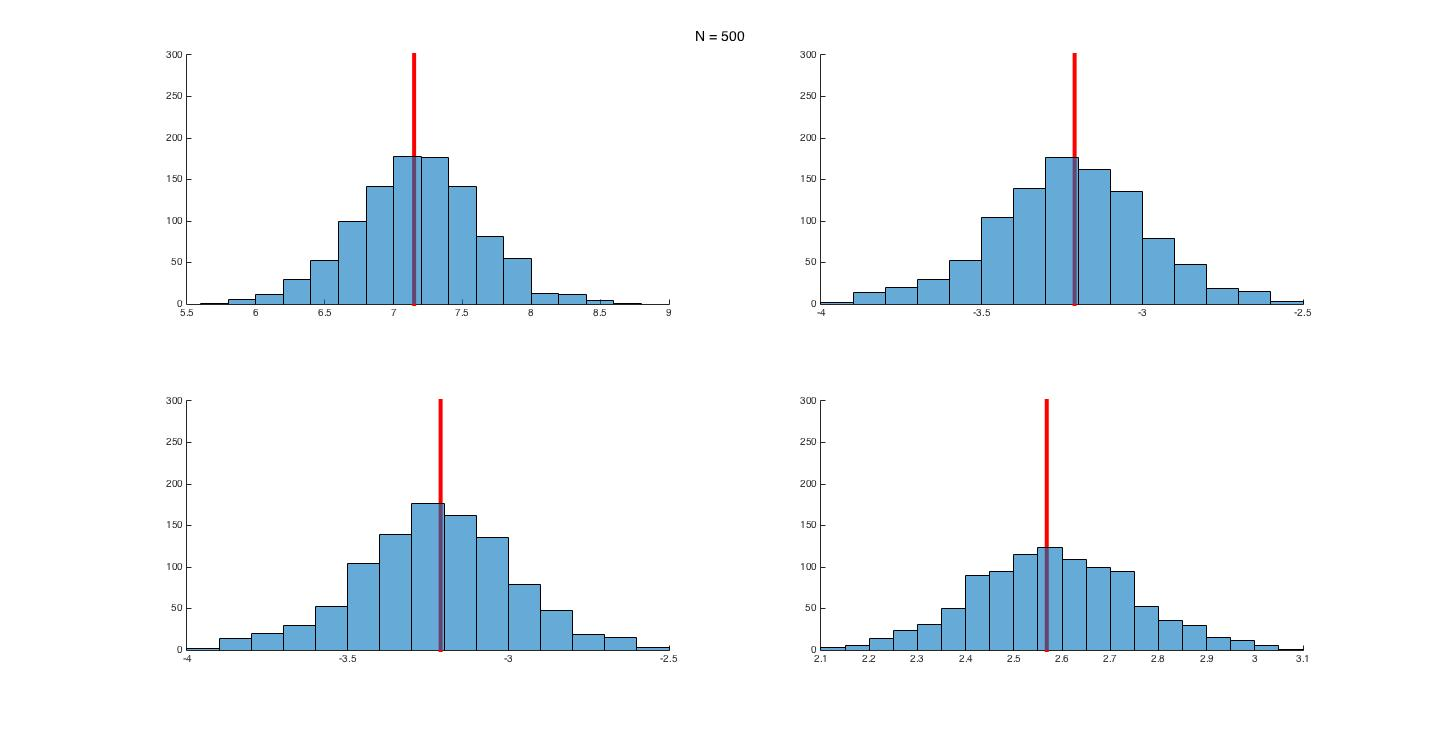
\includegraphics[width=1.2\linewidth]{2b3}
											\caption{1000 samples wishart distribution for N=500}
											\label{fig:2b3}
										\end{figure}																
						\section{Bayesian Inference for the Binomial}
						\subsection*{(a)}
							\paragraph*{Overview}
								Because that $Posterior \propto Likelihood \times Prior$, then $\mu_{MAP}$ can solved by $argmax_{\mu}(Posterior)$.
								\paragraph*{Solve Posterior}
								\begin{align}
								Prior:Beta(\mu|a, b) &= \frac{\Gamma(a + b)}{\Gamma(a)\Gamma(b)}\mu^{a-1}(1-\mu)^{b-1}\\
								Likelihood:Bin(m_{1}|N,\mu) &= \binom{N}{m_{1}}\mu^{m_{1}}(1-\mu)^{N-m_{1}}
								\end{align}
								By (15), (16), we can get $Posterior \propto \mu^{m_{1}+a-1}(1-\mu)^{m_{2}+b-1}, m_{2} = N - m_{1}$
									\paragraph*{Solve $\mu_{MAP}$}
									To $argmax_{\mu}(Posterior)$, we first log Posterior, 
									get $(m_{1}+a-1)\log(\mu)+(m_{2}+b-1)\log(1-\mu)$.
									Then, $\frac{\partial{\mu_{MAP}}}{\partial{\mu}} = 0$, we get $\mu_{MAP} = \frac{m_{1}+a-1}{m_{1}+m_{2}+a+b-2}$
						\paragraph*{(b)}\mbox{}\\
							\begin{figure}[H]
								\centering
								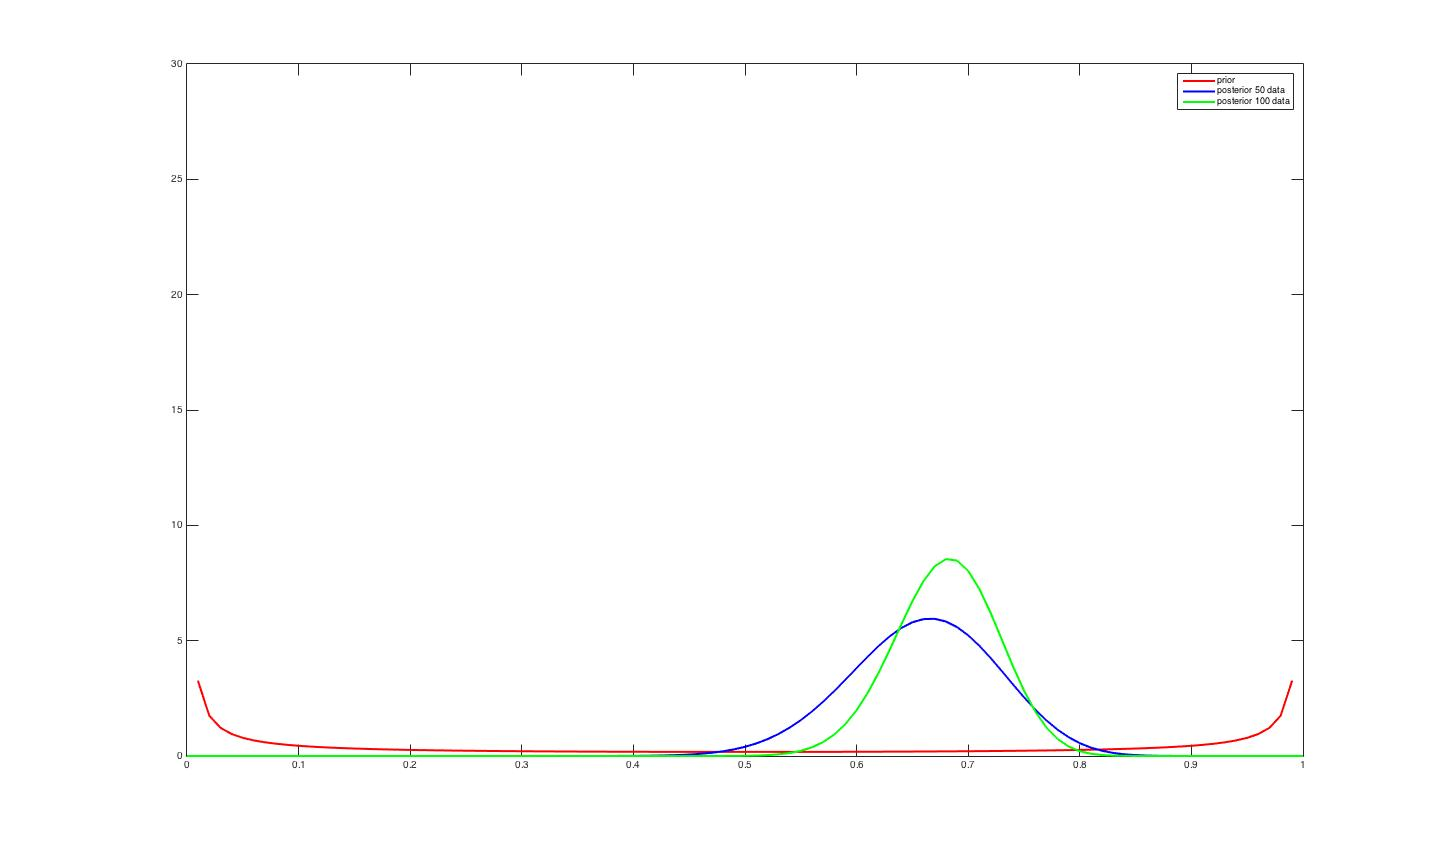
\includegraphics[width=1.2\linewidth]{3a2}
								\caption{prior distribution and posterior distribution for 50 data and all data respectively}
								\label{fig:3a2}
							\end{figure}
\end{document}
